Roots is a holistic system for application performance monitoring (APM), 
performance anomaly detection, and root cause analysis.
It is operated by the cloud providers as a builtin PaaS service that collects data from
all the cloud components user applications interact with. Data collection, storage
and analysis all take place within the cloud, and the insights gained are communicated
to both the cloud administrators and application developers as needed.
The key intuition behind Roots is that, as an intrinsic PaaS service, Roots
has visibility into all activities of the PaaS cloud, across layers.
Moreover, since the PaaS applications we have observed spend most of their time in 
PaaS kernel services~\cite{Jayathilaka:2015:RTS:2806777.2806842}, we hypothesize
that we can infer application performance from observations of how
 the application uses the platform, i.e. by efficiently monitoring the time spent in 
PaaS kernel services. If we are able to do so, then we can avoid application
instrumentation and its downsides, while detecting performance anomalies and 
identifying their root cause quickly and accurately.

The PaaS model that we assume with Roots is one 
in which the clients of a web application engage in a
``service-level agreement'' (SLA)~\cite{Keller:2003:WFS:635430.635442}
with the ``owner'' or operator of the application that is hosted in a PaaS cloud.  The SLA
stipulates a response-time ``service-level objective'' (SLO) that, if violated, 
constitutes a breech of the agreement.
If the performance of an application deteriorates to the
point that at least one of its SLOs is violated, we treat it 
as an \textit{anomaly}. Moreover, we refer to the process
of diagnosing the reason for 
an anomaly as \textit{root cause analysis}.
For a given anomaly, the root cause could be a change in the application workload or
a \textit{bottleneck} in the application runtime. Bottlenecks may occur in the 
application code, or in the PaaS kernel services that the application relies on.

Roots collects performance data across the cloud platform stack, and aggregates it based on 
request/response.  It uses this data to infer application performance, and to identify
SLO violations (performance anomalies).  Roots can further handle different types of anomalies
in different ways.  We overview each of these functionalities in the remainder of this section.

\subsection{Data Collection and Correlation}

We must address two issues when designing a monitoring framework for
a system as complex as a PaaS cloud.
\begin{enumerate}
\item Collecting data from multiple different layers.
\item Correlating data collected from different layers.
\end{enumerate}

%Any PaaS APM must (i) collect data from all layers of the PaaS software stack, and
%(ii) correlate related events across layers.
Each layer of the cloud platform is only able to collect data regarding the
state changes that are local to it. A layer cannot monitor state changes
in other layers due to the level of encapsulation provided by layers. However,
processing an application request involves cooperation of multiple layers. 
To facilitate system-wide monitoring and
bottleneck identification, we must gather data from all the different layers involved
in processing a request. To combine the information across layers
we correlate the data, and link events related to the same request together.

To enable this, we augment the front-end server of the cloud platform. 
Specifically, we have it tag incoming application requests with unique identifiers.
This request identifier is added to the HTTP request as a header, which is visible to all 
internal components of the PaaS cloud. Next, we configure data collecting agents 
within the platform to record the request identifiers along with any events they capture. 
This way we record the relationship between application requests, and the resulting
local state changes in different layers of the cloud, without breaking the existing level
of abstraction in the cloud architecture. This approach is also scalable, since the events are
recorded in a distributed manner without having to maintain any state at the data collecting agents. 
Roots aggregates the recorded events by request 
identifier to efficiently group the related events as required during analysis.

\begin{figure}
\centering
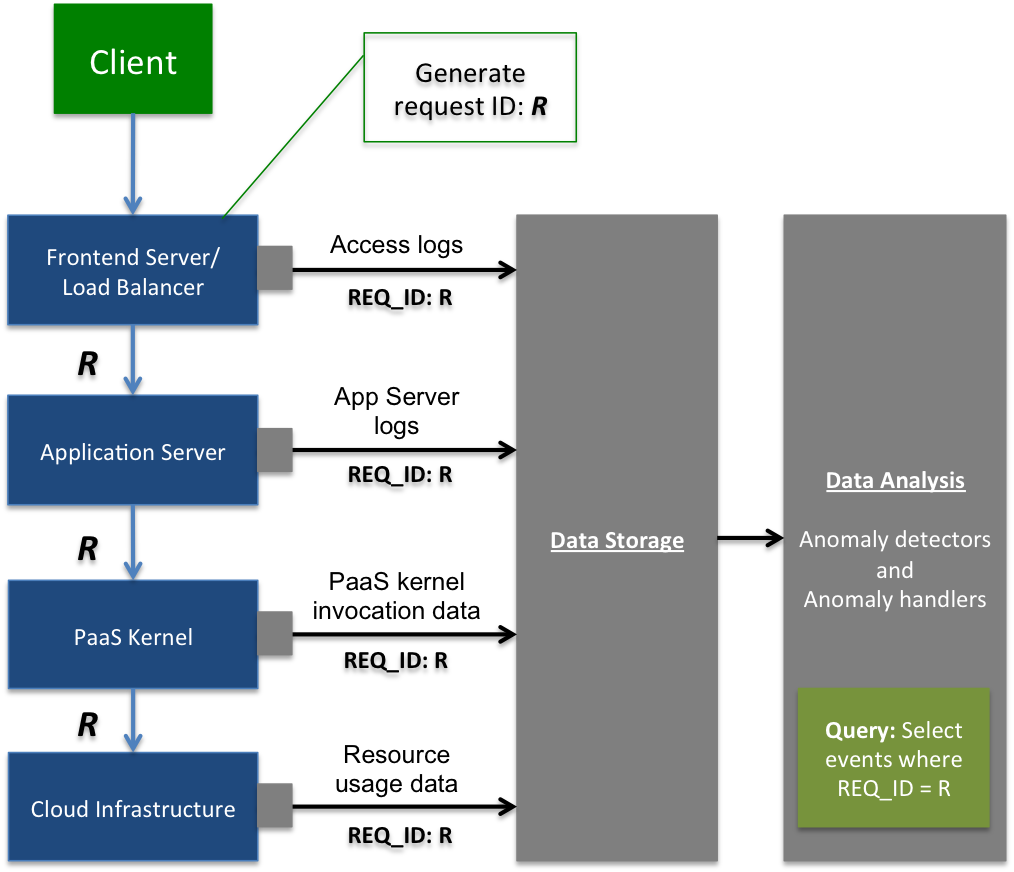
\includegraphics[scale=0.5]{apm_architecture}
\caption{Roots APM architecture.}
\label{fig:apm_architecture}
\end{figure}

Figure~\ref{fig:apm_architecture} illustrates the high-level architecture of Roots, and how 
it fits into the PaaS stack. APM components are shown in grey. 
The small grey boxes attached to the PaaS components represent the
agents used to instrument the cloud platform. 
In the diagram, a user request is tagged with the identifier value
$R$ at the front-end server. This identifier is passed down to the lower layers of the cloud
along with the request. Events that occur in the lower layers while processing this request
are recorded with the request identifier $R$, so Roots can correlate them later. For example, in the 
data analysis component we can run a filter query to select all the events related to a particular
request (as shown in the pseudo query in the diagram). Similarly, Roots can run a ``group by'' 
query to select all events, and aggregate them by the request identifier.

The figure also depicts Roots data collection across the
PaaS stack (i.e. its full stack monitoring). 
From the front-end server, Roots collects
information related to incoming application
requests. It does so by scraping HTTP server access logs, which are
exported by most web servers (e.g. Apache HTTPD or Nginx). 

At the application server level, Roots collects logs and 
metrics related to the application runtime from 
the application servers and operating system.
Roots also employs a set of per-application benchmarking 
processes that periodically probes 
different applications
to measure their performance. These are lightweight, stateless processes 
managed by the Roots framework.
These processes send their measurements to
the data storage component for analysis.

Roots collects information about all kernel invocations
made by the applications by intercepting kernel invocations at 
service interface entrypoints.  For each PaaS kernel invocation, 
we capture the following parameters.
\begin{itemize}
\item Source application making the kernel invocation
\item Timestamp
\item A sequence number indicating the order of PaaS kernel invocations within an application request
\item Target kernel service and operation
\item Execution time of the invocation
\item Request size, hash, and other parameters
\end{itemize}
These PaaS kernel invocation details enable Roots
to trace the execution of application 
requests through the PaaS without instrumenting the application itself.

Finally, at the lowest level Roots collects information 
related to virtual machines, containers
and their resource usage. We gather metrics on network usage 
by individual components which
is useful for traffic engineering use cases. 
We also scrape
hypervisor and container manager logs to track when
resources are allocated and released.

To avoid introducing delays to the application 
request processing flow, we implement
Roots data collecting agents as asynchronous tasks. 
%That is, none of them 
%suspend application request processing to report data to the data storage components.
Agents buffer data locally and periodically write to
data storage components using separate background tasks 
and batch communication
operations. These persistence operations must run 
with sufficient frequency so as to not impede the analysis
that Roots employs to 
detect anomalies soon after they occur.
%We also isolate the activities in the cloud platform from potential
%failures in the Roots data collection or storage components.

\subsection{Data Storage and Analysis}

Roots stores all collected data in a database capable of 
efficient persistent storage
and querying. We facilitate this via indexing
data by application ID and timestamp.
Roots also performs periodic garbage collection on data that is no longer
pertinent to analyses.

The data analysis components consist of two extensible
abstractions: \textit{anomaly detectors} 
and \textit{anomaly handlers}.
Anomaly detectors are processes that periodically 
analyze the data for
each deployed application. 
Roots supports multiple detector implementations, 
each of which is a statistical method for detecting 
performance anomalies. Detectors are configured
on a per-application basis, making it possible for different applications to use different anomaly 
detectors. Roots also supports multiple concurrent anomaly detectors for 
the same application, which can be used
to compare the efficacy of different detection strategies concurrently.
Each anomaly detector has configurable parameters for execution schedule 
and sliding window duration.
We use a period 60 seconds for the former and the previous
hour for the latter, in our prototype and evaluation.
Window size impacts the time range of events processed
by the detector when invoked.
We employ a fixed-size window to bound Roots memory use.

When an anomaly detector detects an anomaly 
in application performance, it sends an event
to a collection of anomaly handlers. 
The event encapsulates a unique anomaly identifier, 
timestamp, application identifier and the source detector's sliding window that correspond to the
anomaly. Anomaly handlers are configured globally (i.e. each handler
receives events from all detectors), but each handler filters events
of interest.
Handlers can also trigger events, which are delivered to
all the listening anomaly handlers. Similar to detectors, 
Roots supports multiple anomaly handler
implementations, e.g., one for logging anomalies, one for sending alert emails, one
for updating a dashboard, etc. 
Additionally, Roots provides two special anomaly handlers:
a workload change analyzer and a bottleneck identifier.
Communication between detectors and handlers 
is performed via shared memory.

The ability of anomaly handlers to filter the events they 
process and to trigger events directly
facilitates construction of 
elaborate event flows with sophisticated logic. For example, the workload
change analyzer can run some analysis upon receiving an anomaly event
from any anomaly detector. If an anomaly cannot be associated 
with a workload
change, it can trigger a different type of event. 
The bottleneck identifier, can
be configured to execute only when such an event occurs.
Using this mechanism, Roots performs workload change analysis first
and systemwide bottleneck identification only when necessary.

%Both the anomaly detectors and anomaly handlers 
%work with fixed-sized sliding windows.
%Therefore, the amount of state these entities must keep in memory has
%a strict upper bound. 
%The extensibility of Roots is primarily achieved through the abstractions of anomaly
%detectors and handlers. Roots makes it simple to implement new detectors and handlers,
%and plug them into the system. Both the detectors and the handlers are executed
%as lightweight processes that do not interfere with the rest of the processes in
%the cloud platform. 

\subsection{Roots Process Management}
\label{sec:process_mgt}

\begin{figure}
\centering
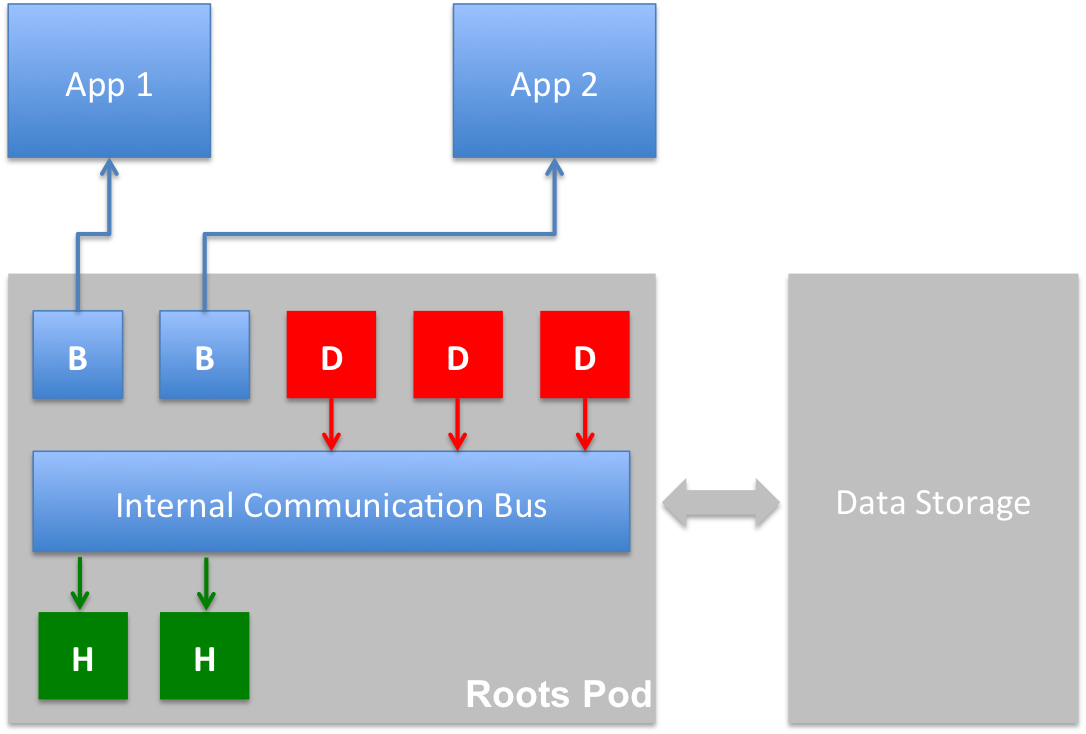
\includegraphics[scale=0.45]{roots_pod}
\caption{Anatomy of a Roots pod. The diagram shows 2 application benchmarking processes (B), 
3 anomaly detectors (D), and 2 handlers (H). Processes communicate via a shared
memory communication bus local to the pod.}
\label{fig:roots_pod}
\end{figure}
Most data collection activities in Roots can be treated as passive -- i.e. they
happen automatically as the applications receive and process requests in the cloud
platform. They do not require explicit scheduling or management. In contrast,
application benchmarking and data analysis are active processes that require
explicit scheduling and management.  This is achieved by grouping benchmarking
and data analysis processes into units called Roots pods. 

Each Roots pod is responsible for starting and maintaining a preconfigured set of
benchmarkers and data analysis processes (i.e. anomaly detectors and handlers). 
These processes are light enough, so as to pack a large number of them
into a single pod. Pods are self-contained entities, and there is no inter-communication
between pods. Processes in a pod can efficiently communicate with each other 
using shared memory, and call out to the central Roots data storage to retrieve 
collected performance data for analysis. 
%This enables starting and stopping 
%Roots pods with minimal impact on the overall monitoring system. 
Furthermore, pods
can be replicated for high availability, and application load can be distributed
among multiple pods for scalability.

Figure~\ref{fig:roots_pod} illustrates a Roots pod monitoring two applications.
It consists of two benchmarking processes, three anomaly detectors and 
two anomaly handlers. The anomaly detectors and handlers are shown communicating
via an internal shared memory communication bus. 

%To automate the process of managing pods, they can be tied into the core
%process management framework of the PaaS cloud. That way whenever the cloud
%platform initializes, a collection of pods can be started automatically.
%Application deployment process of the PaaS cloud can be augmented
%to register each new application with one of the available pods, so that the
%benchmarkers and anomaly detectors can start running on the application.
%Moreover, pods can be moved around or restarted as needed in response
%to errors and autoscaling events that occur in the cloud platform.
